\documentclass[11pt, a4paper]{article}
\usepackage{amsmath, amsfonts, dsfont, booktabs, graphicx, natbib, a4wide, times, microtype, float}
\begin{document}
\title{Solution to Exercise 1}
\author{Simon A.\ Broda}
\date{}
\maketitle
\begin{enumerate}
\item 
\begin{enumerate}
\item  Double-clicking the \texttt{co2} series followed by \texttt{View$\rightarrow$Graph} results in the graph below.
\begin{center}
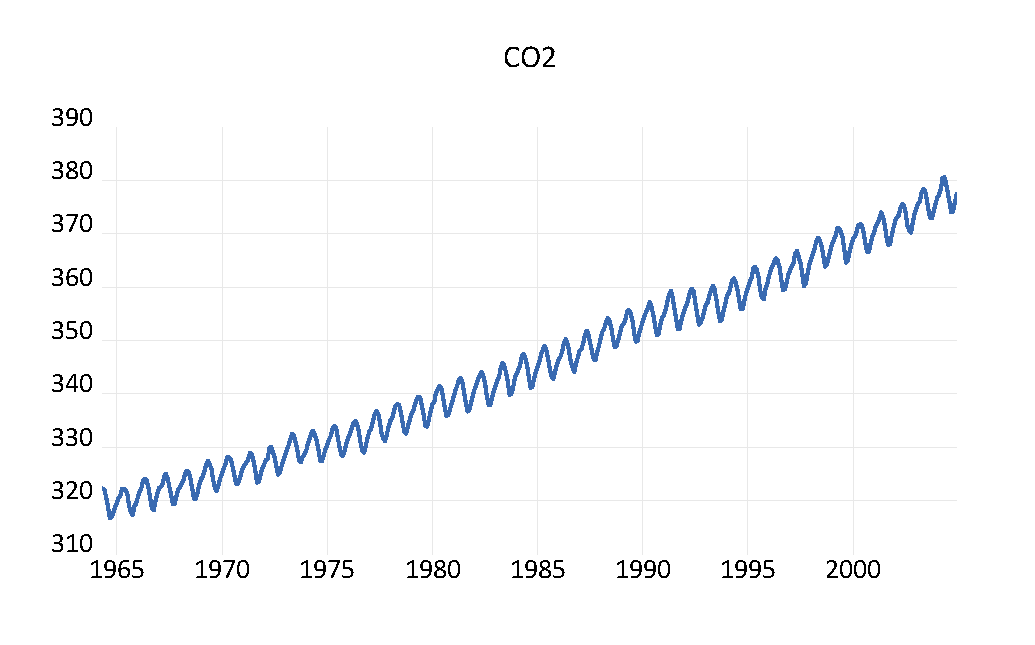
\includegraphics[height=7cm]{co2}
\end{center}
\item Click on \texttt{Quick$\rightarrow$Estimate Equation} and enter the dependent variable, followed by the independent variables, as follows: \texttt{co2 c time}. Here, \texttt{c} stands for a constant (intercept) and \texttt{time} is the variable \texttt{time} from the dataset (take a look at it). Alternatively to \texttt{time}, you can also write \texttt{$@$trend}. This is an EViews function that
generates the trend automatically (in fact, it's how I created the \texttt{time} variable, by writing \texttt{genr time = @trend} in the command window up top).
\begin{center}
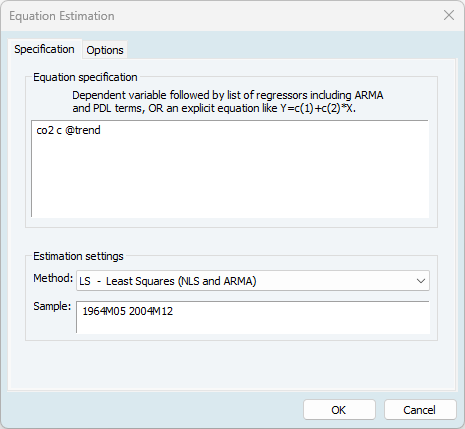
\includegraphics[height=7cm]{linear1}
\end{center}
The result is
\begin{center}
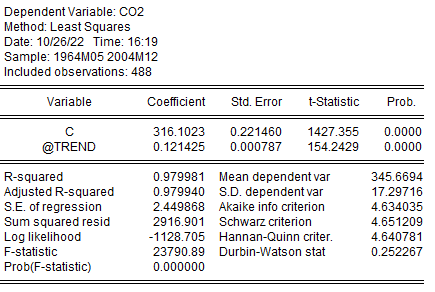
\includegraphics[height=7cm]{linear2}
\end{center}
\item Inside the window with the regression output, go to\\\texttt{View$\rightarrow$Actual-Fitted-Residual$\rightarrow$Actual-Fitted-Residual Plot}. This results in the follow graph.
\begin{center}
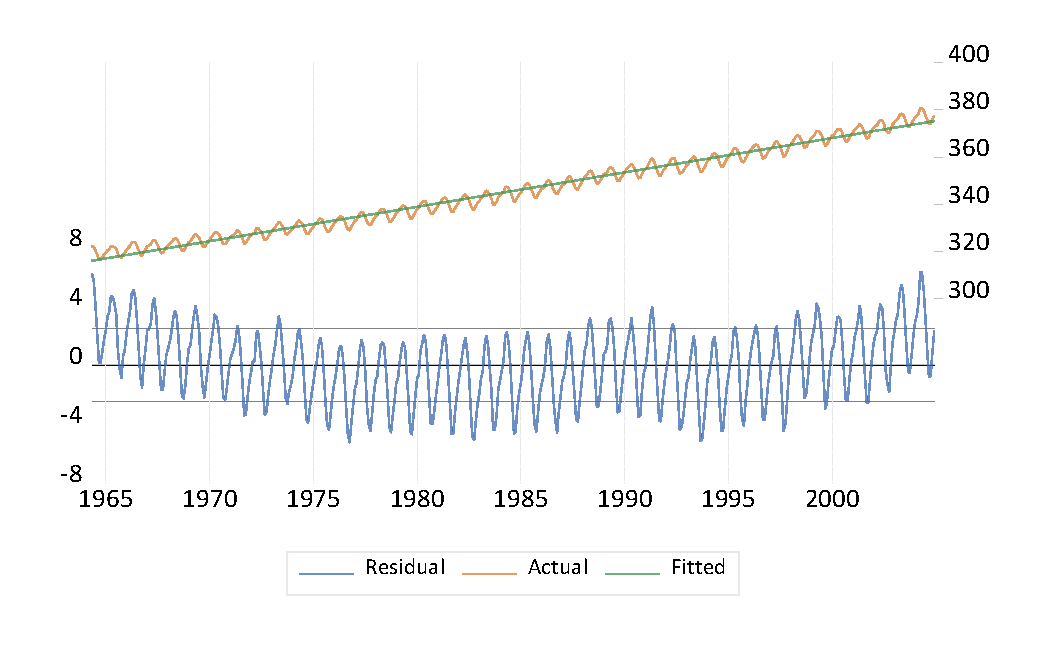
\includegraphics[height=7cm]{linear3}
\end{center}
\item 2005M1 corresponds to $t=488$. Plugging this into the fitted regression
\[\widehat{Y_t}=316.1+0.121\cdot t,\] one obtains
\[\widehat{Y_{488}}=316.1+0.121\cdot 488=375.148.\]
Alternatively, inside the workfile pane on the left, go to \texttt{Proc$\rightarrow$Structure / Resize Current Page\ldots}, and resize the file so that it includes 2005:
\begin{center}
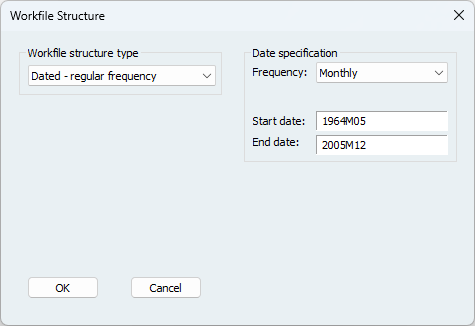
\includegraphics[height=7cm]{resize}
\end{center}
Then, inside the window with the estimation output, click on \texttt{Proc$\rightarrow$Forecasts\ldots}, and extend the forecast sample to 2005M12.
\begin{center}
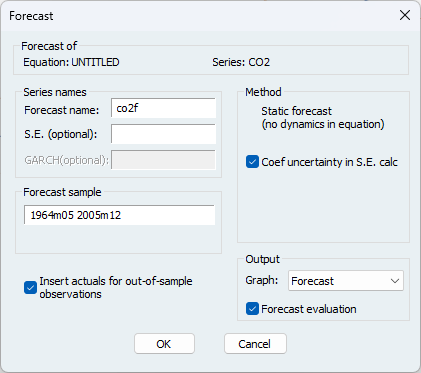
\includegraphics[height=7cm]{forecast}
\end{center}
Finally, open the \texttt{co2f} series and find the value corresponding to 2005M1; it's {375.358}. The difference is due to the fact that EViews uses the unrounded estimates.
\item Estimating \verb+co2 c @trend @trend^2+ yields
\begin{center}
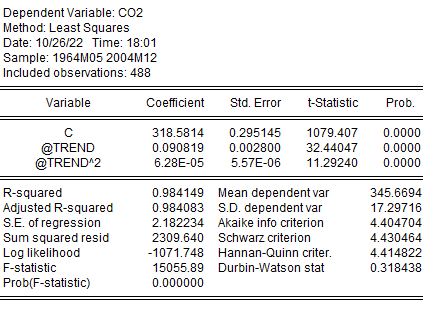
\includegraphics[height=7cm]{quadratic1}
\end{center}
and
\begin{center}
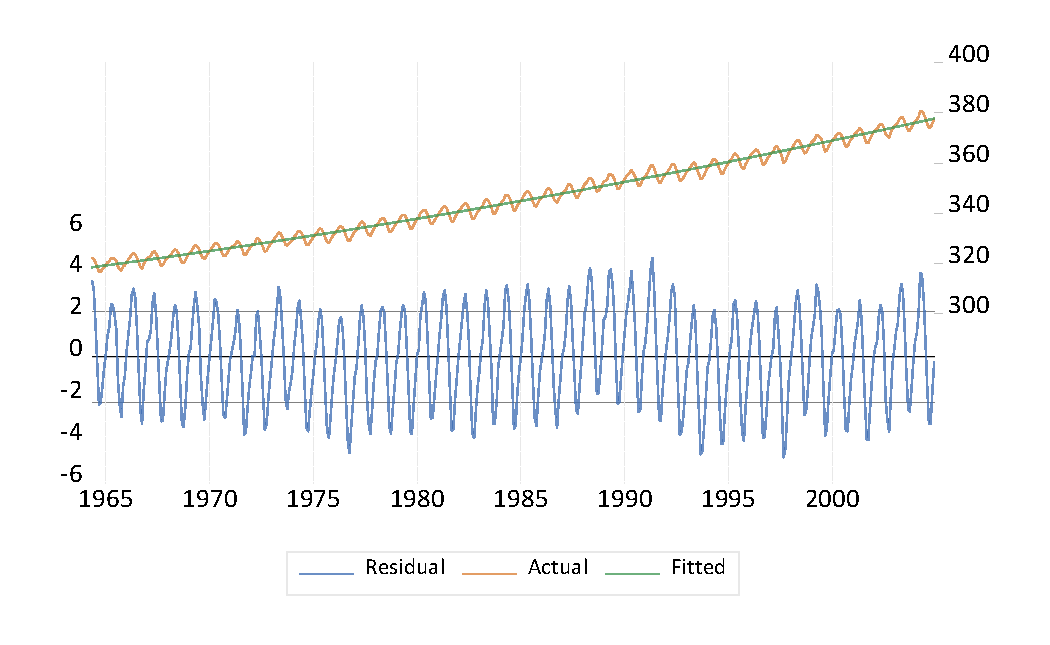
\includegraphics[height=7cm]{quadratic2}
\end{center}
Eyeballing, the resulting fit looks better; also, there is less structure in the residuals. The forecast is
\[\widehat{Y_{488}}=318.58+0.09\cdot 488+0.0000628\cdot488^2\approx 377.868.\]
\item First, we have to take logs of the dependent variable: in the command window up top, write \texttt{genr logco2 log(co2)} (\texttt{genr} stands for generating a new series; \texttt{log} is the natural logarithm). This creates a new series \texttt{logco2}. Next, regress this new variable on a constant and the time trend using \verb+logco2 c @trend+. This yields
\begin{center}
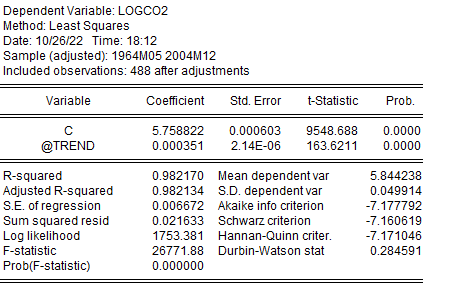
\includegraphics[height=7cm]{exponential1}
\end{center}
The estimated parameters of our exponential trend
\[
F_t = \beta_0\cdot\beta_1^t
\]
are $\widehat{\beta_0}=\exp(5.758822251222528)=316.97$ and $\widehat{\beta_1}=\exp(0.0003507827256490508)=1.0003508442571039$, implying that atmospheric CO2 increases by 0.035\% a month, or $1.035^{12}-1=0.42$\% a year. The forecast for 2005M1 is
\[
\widehat{Y_{488}}=316.97\cdot 1.0003508442571039^{488}=376.15.
\]
%Note: instead of transforming the data to logs for linearization and then applying OLS, it is also possible to have EViews estimate an exponential model directly, by entering \verb.co2 @exp(c(1) + c(2) * @trend). as the model specification. This also allows us to do the plots and the forecasting directly in EViews as with the linear and quadratic models. It results in slightly different parameter estimates because EViews uses a different algorithm in place of OLS. The resulting forecast is $\widehat{Y_{488}}=376.28$, and the plot looks as follows.
%\begin{center}
%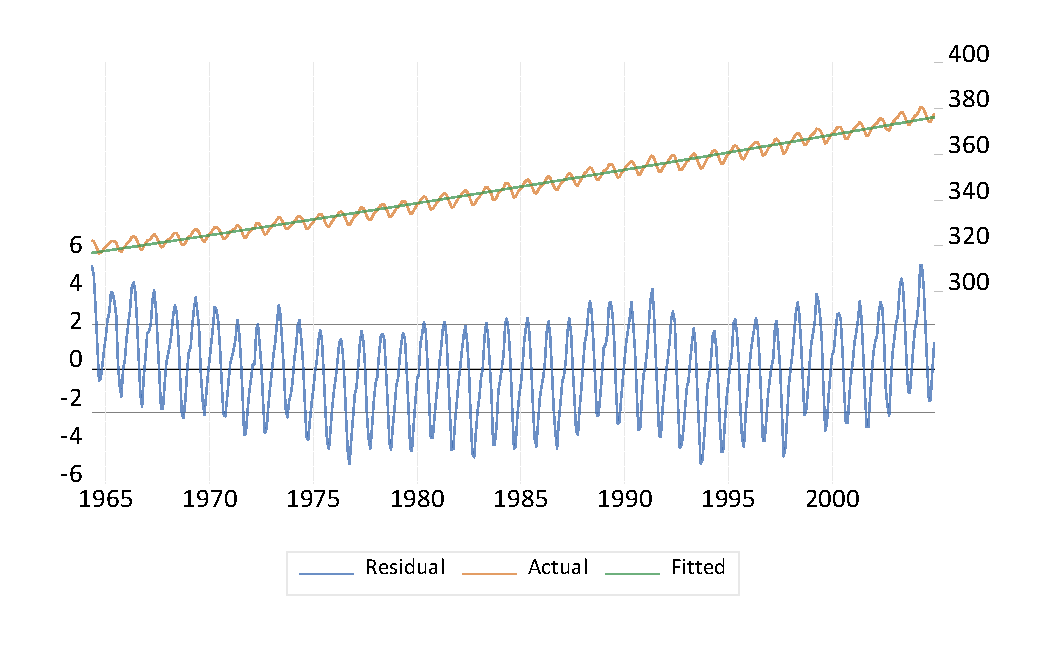
\includegraphics[height=7cm]{exponential2}
%\end{center}
\end{enumerate}
%The fit looks worse than our quadratic model from earlier.
\item 
\begin{enumerate}
\item We obtain
\[
(322.23+321.89+320.44)/3 = 321.52.
\]
\item Enter \verb.genr ma12 = @movavc(co2, 12). in the command window (\verb.@movavc. stands for a centered moving average). For the plot, select both series with the mouse (press \texttt{CTRL} while clicking to select both), then right-click and select \texttt{Open$\rightarrow$As Group}, and plot as usual. This results in the following plot.
\begin{center}
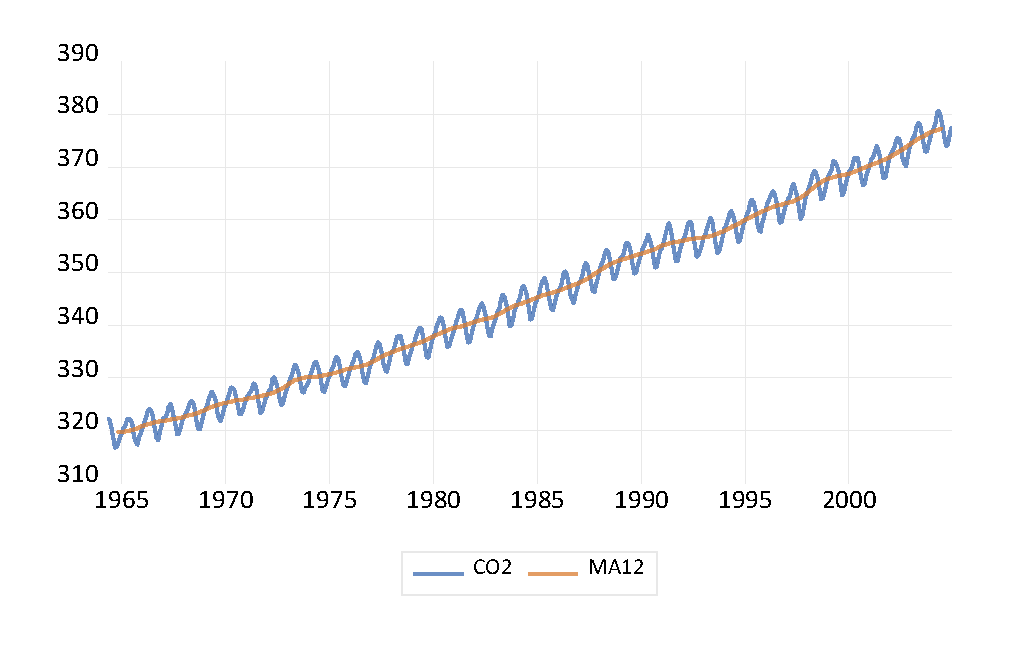
\includegraphics[height=7cm]{ma12}
\end{center}
\end{enumerate}
\item
\begin{enumerate}
\item Rather than constructing the dummies manually, we can have EViews construct them automatically for us, by entering the equation as \verb.co2 @trend @expand(@month). (for quarterly data, we would use \verb+co2 @trend @expand(@quarter)+, etc.). This results in the following output:
\begin{center}
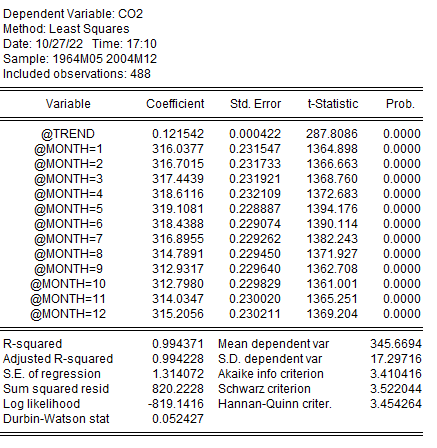
\includegraphics[height=7cm]{seasonal1}
\end{center}
The forecast for 2004M12 is
\[
\widehat{Y}_{487} = 0.121542\cdot487+315.2056=374.397,
\]
which can also be obtained via \texttt{Proc$\rightarrow$Forecasts\ldots}. The actual-fitted-residual plot is given below.
\begin{center}
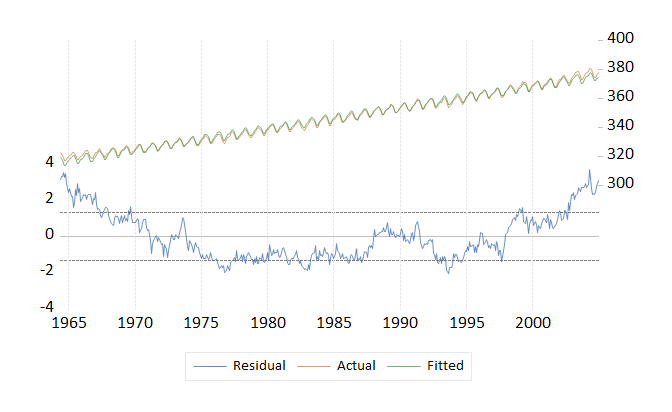
\includegraphics[height=7cm]{seasonal2}
\end{center}
As we had discovered earlier, there is still structure left in the residuals; a quadratic trend is a better fit. Including a quadratic term (not asked) yields the following:
\begin{center}
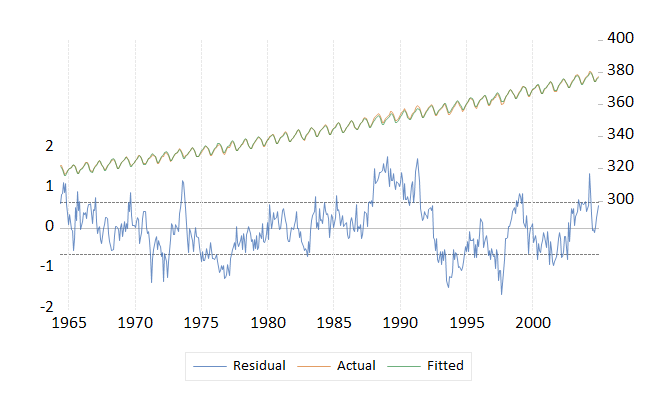
\includegraphics[height=7cm]{seasonal3}
\end{center}
\item Now we use the specification \verb.co2 c @trend @expand(@month, @droplast).. This yields the following output.
\begin{center}
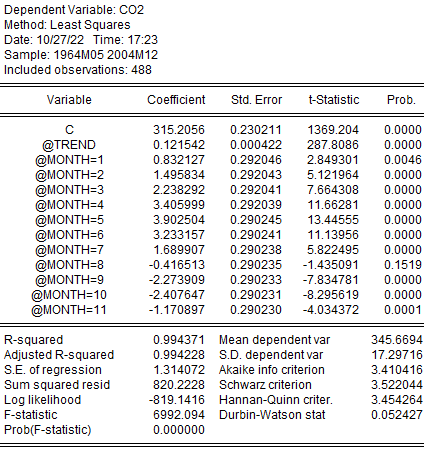
\includegraphics[height=7cm]{seasonal4}
\end{center}
Notice how December is now the base case with an average of 315.2, and all other months are measured in relation to it.
The forecast for 2004M12 is
\[
\widehat{Y}_{487} = 315.2056+0.121542\cdot487=374.397,
\]
the same as before.
\end{enumerate}
\end{enumerate}
\end{document} 